% This file is for the problem formulation section of the Master's Thesis.
% This file will not compile on it's own. Will need to include it into a main file
% That uses the drexel thesis template.
\chapter{Problem Formulation}

Detecting frame deletion in a video requires detecting the structural changes in a video due to the deletion process. In particular, Wang and Farid's work on temporal traces for detecting frame deletion shows that for MPEG-2 video, the P-frame prediction error can be formulated into a sequence, which can be monitored to detect frame deletion. Both Wang and Farid, and Stamm use a system like in Fig. ~\ref{System} to detect frame deletion. The prediction error sequence $e(n)$ is extracted from the decoded video file and processed to produce detection features. Wang and Farid's work did not propose features for automatic detection, and instead relied on visual inspection of the DFT of the prediction error sequence.

\begin{figure}[htbp]
\centerline{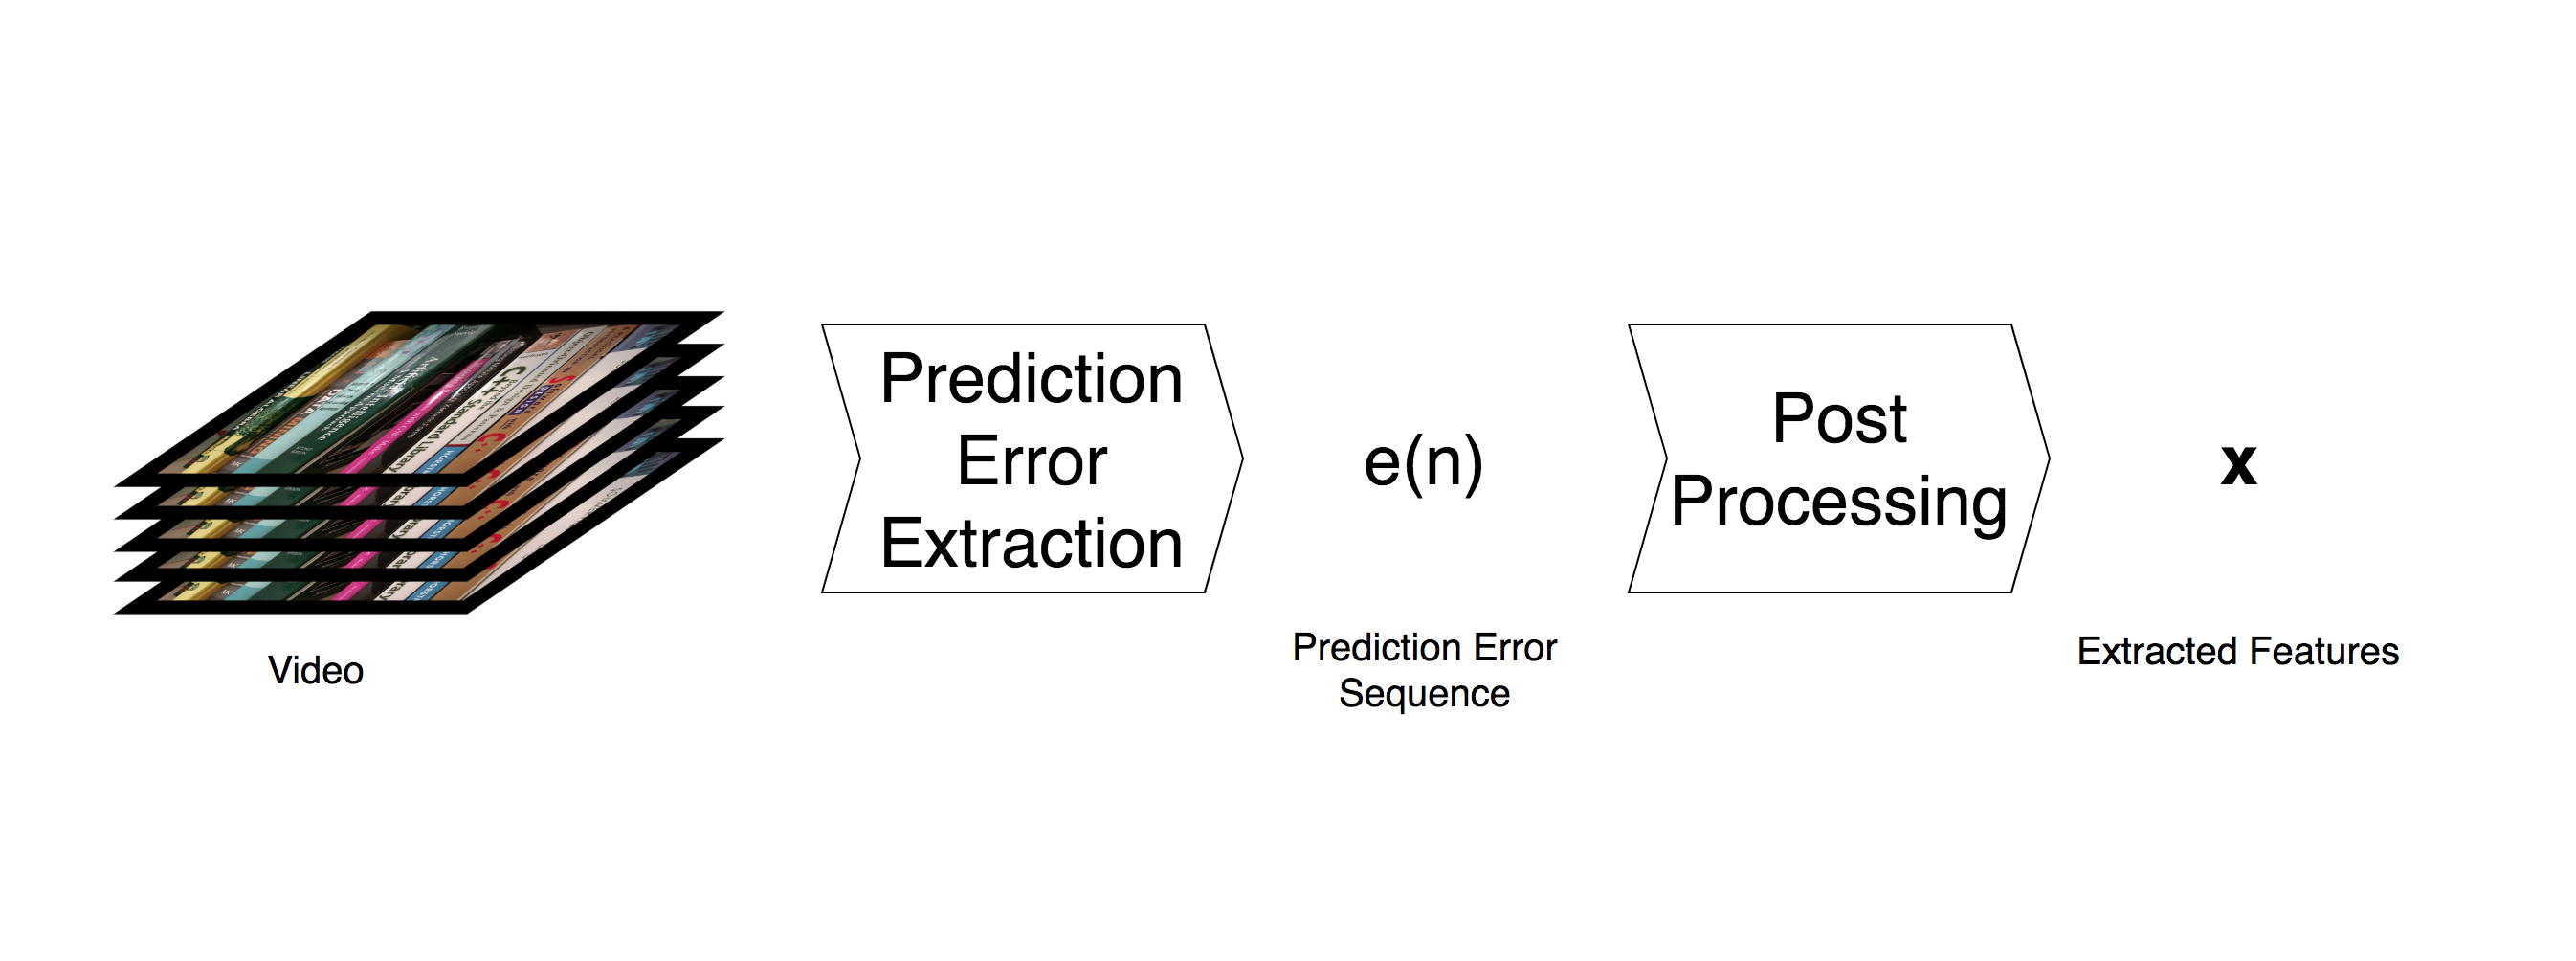
\includegraphics[width=0.9\linewidth]{ProblemFormulation/frame_deletion_detection_system.png}}
\caption{Generalized System for Frame Deletion Detection}
\label{System}
\end{figure}

This generalized system will also work with H.264 encoded video as well. While video encoding has advanced significantly, the fundamental structures of a compressed digital video have remained unchanged. Videos are still stored in GOPs with different numbers of I, P, and B-frames. However, the prediction error extraction and post processing steps must be altered or augmented to remain robust to said advances in video compression.

As this work is concerned particularly with the detection of frame deletion in H.264, we have made the following assumptions. First, we assume that all altered video has undergone re-compression. In fact, since most consumer video recording devices do not have the storage capability or processing power to record high-definition raw video, it is assumed that all video sources have been compressed by either MPEG-4 or H.264, and that all frame deleted video will be re-compressed using H.264, where the reencoding is set to match the GOP structure of the source video. 

In addition, it is assumed that all videos that are passed to the detector are of sufficient length to make a classification. Without multiple full GOPs, the presence of a deletion fingerprint is negligible. Lastly, we make the assumption that if indeed frames have been removed from a video, they have not been removed from the end of the video. The detection features are dependent on differences between the structure of the prediction error sequences in natural videos versus videos with frame deletion. When frames are removed from the end of the video sequence, this difference is not observable.

A user of our proposed system will not need physical access to a specific device to analyze a video captured by the device. The system should accept videos of an arbitrary length, and will not require metadata unrelated to video playback to be in tact. It will work with videos of any resolution, frame rate, or GOP structure. Also, as our approach will be data driven, it is imperative that a user have access to a sufficient database of videos with known labels.

\section{Video Frame Deletion Detection}

Detecting frame deletion is a binary classification problem. Given a Video $V$, there are two possible classes:

\begin{equation}
\begin{aligned}
  C_{0} &: \text{The video is genuine, and has not had frames removed from it.} \\
  C_{1} &: \text{The video is altered, and has had frames removed from it.}
\end{aligned}
\end{equation}

Note that in this case, \emph{genuine} refers to the fact that the video has not undergone any frame deletion. A video may have underwent other post processing operations such as color correction and re-sizing but not have had any frames removed. In this case, the video would be said to be genuine. From this point forward, any mention of a genuine video simply refers to a video that has not had frames removed from it.

In general, it is difficult to classify based on the entirety of a video directly, thus the problem must be reworked. As shown above, a feature extraction system will be used to produce the P-frame prediction error sequence $e(n)$, and a feature vector $\bm{x}$. The feature vector ideally contains information about the prediction error sequence that can perfectly separate the two classes. As such, the classification problem is as follows. Given a feature vector $\bm{x}'$, it belongs to one of two classes:

\begin{equation}
\begin{aligned}
  C_{0} &: \bm{x}' \text{resulted from a genuine video that has not had frames removed from it.} \\
  C_{1} &: \bm{x}' \text{resulted from an altered video which has had frames removed from it.}
\end{aligned}
\end{equation}

In the following chapter, we will propose both a new method for extracting $e(n)$, and additional augmentations to $\bm{x}$ that allow for improved separation of data and increased robustness of the overall system.
